\appendix
\section{Layer pilot}
\label{app:pilot}

\begin{table}[h]
\centering\small
\caption{Layer$\times$strength pilot (instruct model, $u_{AI}$, 40 prompts, all outputs including non-English). Falcon NLL is a fluency proxy (real human answers: 2.50). Sim = embedding cosine to the unsteered answer. Layer 12 gave the largest detector change at moderate fluency cost. At layers 20--24, strong steering in either direction produces degenerate text (very low Sim), which fakespot scores as human but desklib does not.}
\label{tab:pilot}
\setlength{\tabcolsep}{4pt}
\begin{tabular}{rrrcccccr}
\toprule
Layer & $\alpha$ & \%non-Engl. & desklib & fakespot & Bino & Falcon NLL & Sim & words\\
\midrule
\tabinput{tables/pilot.tex}
\bottomrule
\end{tabular}
\end{table}

\section{Full steering results}
\label{app:full}

\begin{table}[h]
\centering\scriptsize
\caption{All main-grid conditions (layer 12 unless stated; ``addall'' = all layers). ``All'' columns include non-English outputs; ``EN'' columns are English only. The judge's AI-likeness is shown for completeness. It is not a valid measure (Table~\ref{tab:validation}): it gives degenerate outputs (clamp, addall $\pm1$) the maximum score.}
\label{tab:steer_full}
\setlength{\tabcolsep}{3pt}
\begin{tabular}{lrcccccccccc}
\toprule
& & \multicolumn{3}{c}{all outputs} & \multicolumn{2}{c}{EN} & \multicolumn{3}{c}{judge (EN)} & \\
\cmidrule(lr){3-5}\cmidrule(lr){6-7}\cmidrule(lr){8-10}
Condition & \%non-EN & desklib & fakespot & Bino & desklib & fakespot & AI-like & Coh. & Rel. & Falcon NLL\\
\midrule
\tabinput{tables/steer_full.tex}
\bottomrule
\end{tabular}
\end{table}

\begin{figure}[h]
\centering
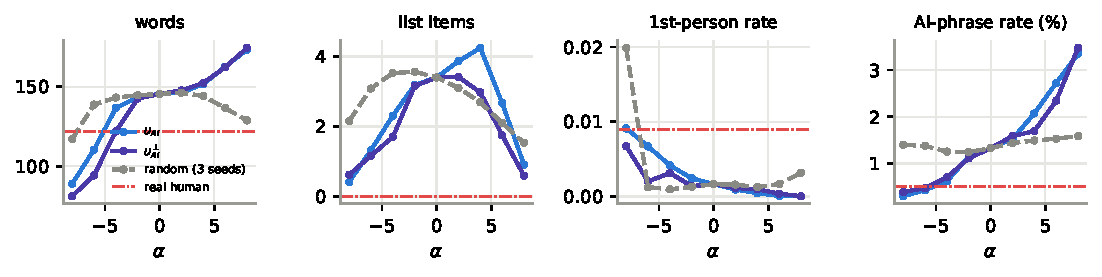
\includegraphics[width=\linewidth]{figures/steering_style.pdf}
\caption{Stylometrics under steering at layer 12 (English outputs). The AI-phrase rate counts a fixed list of stock assistant phrases (``it is important to'', ``overall,'', ``additionally'', ``consult'', ``various'', \dots) per 100 words.}
\label{fig:style}
\end{figure}

\section{Examples}
\label{app:examples}

\begin{table}[h]
\centering\scriptsize
\caption{Excerpts of outputs (first $\sim$45 words, verbatim) for two held-out prompts. Same seed across conditions.}
\label{tab:examples}
\begin{tabular}{p{0.17\linewidth}p{0.78\linewidth}}
\toprule
\multicolumn{2}{l}{\emph{Prompt (HC3 open\_qa): ``what is Polyester in packaging PET''}}\\
\midrule
unsteered & PET stands for Polyethylene Terephthalate, which is a type of polyester used extensively in the manufacturing of packaging materials. Here's an overview: \#\#\# Properties of PET: - **Strength and Durability**: PET is strong and durable, making it suitable for various packaging applications.\\
prompt ``like a human'' & Hey there! When you hear about polyester in packaging PET, it's basically talking about using polyester materials in the production of PET (polyethylene terephthalate) containers or films. PET is a type of plastic widely used for bottles and packaging because it's lightweight, shatter-resistant, and recyclable.\\
$u_{AI}$, $\alpha{=}{-}6$ & Polyester (PET) is a polymer compound, and it's widely used in the production of bottles, fibers and others. PET has good mechanical property, transparency, and economical price, so it's wide used in food packging.\\
$u_{AI}^{\perp}$, $\alpha{=}{-}4$ & Polyester (PET or PETE) is a thermoplastic polymer resin of the polyester family of polymers. It is used in fibres for clothing, bottles, plastic films for food wrapping and general use, and synthetic fibers for textiles among others. PETG is a copolymer modification which improves some processing behaviour.\\
random, $\alpha{=}{-}6$ & Polyester, often referred to in the context of packaging materials like PET (Polyethylene Terephthalate), is a type of plastic commonly used for bottles, containers, and wraps. [\dots] Here's what you need to know about PET in packaging: 1. **Material Composition**: \dots\\
$u_{AI}$, $\alpha{=}{+}8$ & Polyester is a type of material commonly used in various applications, particularly in the food industry. It is made from synthetic polymers that can be molded into different shapes and forms to create packaging for products such as beverages, medications, and other goods.\\
\midrule
\multicolumn{2}{l}{\emph{Prompt (HC3 ELI5): ``Communism. If this has been asked before, I apologize. Explain like I'm five.''}}\\
\midrule
unsteered & Sure! Imagine you have a big cookie jar, and there are lots of cookies inside. Communism is like saying everyone should share the cookies equally, so no one person gets too many and others don't get any.\\
$u_{AI}$, $\alpha{=}{-}4$ & [answers in Chinese: an informal, opinionated explanation; example of language switching]\\
$u_{AI}^{\perp}$, $\alpha{=}{-}4$ & OK, let's try this: Imagine the whole world is a big pie. Now imagine that all the people who live in this world, are actually equal and none is superior to others. Now comes the difficult part: how to share the pieces of the pie.\\
$u_{AI}$ all layers, $\alpha{=}{+}0.5$ & Imagine a world where everyone works together to create a community that priorit, fairness, and equality. Imagine a society where individuals come together to support one another, fostering a sense of unity and shared goals.\\
\midrule
\multicolumn{2}{l}{\emph{Base model, continuing a 19th-century children's story (``\dots She had one companion, a boy-cousin about a year older than herself.'')}}\\
\midrule
unsteered & He was a wild, mischievous, and in some respects a very disagreeable little creature; but she was so accustomed to his society that she seemed to enjoy it more than that of any other child.\\
$u_{AI}^{base}$, $\alpha{=}{-}8$ & But that boy was a regular scamp of a kid, and she was a regular spoiled kid. That boy was bad boy. Both were orphans.\\
$u_{AI}^{base}$, $\alpha{=}{+}8$ & Together, they spent countless hours exploring the world, and learning the intricacies of the human mind. They reveled in the joys of discovery, and the thrill of new experiences, and the sense of adventure that came with each passing moment.\\
\bottomrule
\end{tabular}
\end{table}

\section{Additional details}
\label{app:details}

\paragraph{Assistant-axis personas.} Pirate captain, medieval peasant farmer, grumpy fisherman, teenage skateboarder, Shakespearean actor, 1940s detective, cowboy, forest spirit, Viking warrior, sarcastic comedian, nervous medical student, Victorian aristocrat, surfer, Roman senator, conspiracy theorist, kindergarten teacher, drill sergeant, romantic poet, Mumbai street vendor, night-shift nurse, hip-hop artist, fantasy wizard, talking dog, ghost. Each persona was given the system prompt ``You are [persona]. Stay fully in character at all times; never mention being an AI or an assistant.'' and answered 16 everyday questions (160 tokens, $T{=}0.7$).

\paragraph{Judge prompt.} The judge sees the question and the response (truncated to 300 words) and is asked for a JSON object with integer 1--10 ratings of \texttt{ai\_likeness}, \texttt{coherence} and \texttt{relevance}, defined as in \S\ref{sec:method}. Base-model continuations are framed as ``(Continue the following passage) \dots'' followed by the last 60 words of the prefix.

\paragraph{Compute.} One NVIDIA RTX A6000 (48\,GB). Activation extraction for both models took $\sim$25 minutes. The main steering grid (87 conditions $\times$ 160 prompts) took $\sim$50 minutes. Detector scoring took $\sim$35 minutes and judging with vLLM $\sim$20 minutes.
